%!TEX root = ../template.tex
%%%%%%%%%%%%%%%%%%%%%%%%%%%%%%%%%%%%%%%%%%%%%%%%%%%%%%%%%%%%%%%%%%%%
%% chapter2.tex
%% NOVA thesis document file
% % ================
% % = Introduction =
% % ================
%%15 a 30 páginas  deve citar entre 20 a 40 %%referências.
%% Chapter with the State of the Art
%% 22 pages max
%%%%%%%%%%%%%%%%%%%%%%%%%%%%%%%%%%%%%%%%%%%%%%%%%%%%%%%%%%%%%%%%%%%%
\chapter{State of the Art}
\label{cha:state_of_the_art}
%  ================
%  = Introduction =
%  ================

In this chapter, the state-of-the-art on the main research subjects is presented. 
Firstly, an overview of current Solutions for People with dementia is described, then a review of the main~\gls{IoT} LPWANS, followed by the current trends of the supported emergent LPWANS technologies, finally a comparison table is shown. 
Afterwards, a description of the current Geolocation solutions is provided, along with the advantages and disadvantages of the application of these technologies on the Active and Assisted Living. Concluding with the presentation of the related work on the research topic.

% Section Solutions for People with Dementia Start
\section{Solutions for People with Dementia}
\label{sec:PWD_SOTA}
% 1,2 pages IoT produtos relacionados Quem está  a usar e o que?


The solutions available today  for wearable devices, used as trackers for people with dementia, have a problem which is that continuous GPS tracking devices suffer from reduced battery life. This is caused by the power consumption of the~\gls{GNSS} module,  and the use of cellular networks, such as~\gls{GSM}, that are not optimised for the size and power efficiency needed for this particular use case. 

These devices are  used by caregivers, to reduce  one of the critical risks of people with dementia that is wandering to unsafe areas. At the moment the best device capable of tracking people with dementia,  on the market, as less than 10 hours of battery usage with a big battery.
The problem in this solution is that  requires from the part of the  patients or caregivers a daily battery charging.
The figure~\ref{fig:Device-battery-Comparison}, is based on the one from~\cite{Hadwen2017}, and the devices in June of 2020 are available at the following links \href{https://www.tictoctrack.com.au/}{TicTocTracker}, \href{http://www.bluewatersecurityprofessionals.com/elderlytracking.htm}{BlueWater watch},  \href{https://mcarewatch.com.au/}{mCare watch}, \href{https://gpssmartsole.com/gpssmartsole/}{SmartSole}, the figure shows the battery duration, in live tracking mode and  standby.\newline\newline\newline\newline\newline

\begin{figure}[htbp]
  \centering
  
    {\includegraphics[height=2.8 in,width=0.55\linewidth]{Chapters/Figures/21.png}}%
 
  \caption{Device Battery Comparison}
  \label{fig:Device-battery-Comparison}
\end{figure}

The following table~\ref{tab:PwD-comparison} shows a comparison between the above-mentioned devices, where the price of the product is presented. In the technical part, a comparison of the  geolocation technique  and communication method is also shown. By reading this table the wearable type of these solutions are always similar except in the smart sole, and geolocation is always based on~\gls{GPS}, the communication is cellular except in the TicTocTracker product were WiFi is also an option. The conclusion is that all the solutions are somehow similar, expensive, and not optimized for power efficiency. \newline
\begin{table}[htbp]
\begin{tabular}{lllll}
\hline
Company & GTX & mCare & TicTocTrack & Bluewater \\ \hline
Product & SmartSole & watch & TicTocTracker & Bluewater watch \\
Price & \begin{tabular}[c]{@{}l@{}}272€ Device\\ 23€/month\end{tabular} & \begin{tabular}[c]{@{}l@{}}453€ Device\\ 23-63€/month\end{tabular} & \begin{tabular}[c]{@{}l@{}}182€ Device\\ + SIM Plan\end{tabular} & \begin{tabular}[c]{@{}l@{}}544€ Device\\ 32€/month\end{tabular} \\
\multicolumn{5}{l}{Technical:} \\
Geolocation & GPS & GPS & GPS & GPS \\
Comunication & GSM & 4G & 3G / WiFi & NaN \\
Wearable type & sole & watch & watch & watch \\ \hline
\end{tabular}
\caption{PwD comparison }
\label{tab:PwD-comparison}
\end{table}
% Section Solutions for People with Dementia (end)
\newpage
% Section LPWAN Start
\section{LPWAN} % (fold)
\label{sec:LPWAN}

\textit{"By the year of 2025, up to 75 billion devices would be connected in Internet-of-Things (\gls{IoT}), with a potential economic impact of around 11.1 trillion \$ a year"}~\cite{ LPIkpehai2019}. The need for an~\gls{LPWAN} emerges when M2M communication is necessary and other wireless networks, for example, the ones with a short-range (Bluetooth, RFID, Wifi or Zigbee) are not a good fit for our application,~\gls{LPWAN}s are suited to connect devices that only need to send a small amount of data over a long distance (100m to 15km or more). The key features in all of the  different~\gls{LPWAN} technologies will be a long-range, and low power consumption, for achieving this the data rate will also be low.

\begin{figure}[htbp]
  \centering
  
    {\includegraphics[width=0.6\linewidth]{Chapters/Figures/LPWAN-Positioning.jpg}}%
 
  \caption{LPWAN Position in Range VS Data rate~\cite{Mekki2019}}
  \label{fig:LPWAN_Positioning}
\end{figure}

There are two main types of a network configuration for the~\gls{LPWAN}.
First Mesh Topology, where all nodes are connected in a none structured way, and can communicate with each other, to distribute data amongst each other. Although this is not entirely true for some implementations of this topology, one of the most well known is Zigbee. In this implementation exists three different roles, the coordinator which connect to the internet, the end nodes, and in between the mesh routers, these cooperate to relay the message to the coordinator. 

Second Star topology network is the approach widely used, the end nodes of a star network are connected directly to the gateway, and this gateway is connected to the internet, this is similar to WiFi. In a star topology when there is the  need for  better coverage,  and reliability there is always the possibility to add more repeaters~\cite{LPLinkLabs}.

Besides the network configuration, LPWANS can be further divided into two groups, depending on which part of the wireless spectrum they work on, these groups are Licensed and Unlicensed~\cite{LPZourmand2019}.


% subsection lora_sota Start

\subsection{LoRa} % (fold)
\label{sec:lora_sota}

LoRa is an~\gls{LPWAN} initially developed by the French company Cycleo and later acquired by Semtech. LoRa is a semi-proprietary standard, and is composed of two major components. 

First LoRa that stands for Long Range represented in orange at figure~\ref{fig:lora_intro}, this is the physical layer and it is the proprietary part of the stack. This layer  is based on chirp spread spectrum modulation, which in comparison with other radio technologies maintains the same low power characteristics as FSK (Frequency Fey Shifting) modulation, but with a higher communication range. The CSS has been in use for decades because of the long distances that can be achieved and the immunity to external interference. This technology operates in the~\gls{ISM} bandwidth, in Europe that is 868 MHz. 

The Second LoRaWAN represented in figure~\ref{fig:lora_intro} in blue, is responsible for defining the communication protocol and the system architecture for the network. The protocol and network architecture have a role in determining the battery lifetime of the end device, the quality of service, the network capacity, the security, and the variety of applications served by the network.

\begin{figure}[htbp]
  \centering
    {\includegraphics[width=0.6\linewidth]{Chapters/Figures/introlora.PNG}}%
  \caption{LoRa Stack~\cite{What_is_LoRa}}
  \label{fig:lora_intro}
\end{figure}

In terms of specifications, LoRa as data rates from 300 bps to 50 kbps, this occurs because LoRa as adaptive data Rate, that is dependent of the spreading factor in use, following the next equation:
\begin{equation}
    \label{eq:Modulation_Bit_Rate}
        R_b = SF *  \frac{1}{\frac{2^{SF}}{BW}}\hspace{5mm} bits/sec
\end{equation}
In the previous equation:
\begin{itemize}
	\item {$R_b$} - Bitrate
	\item SF - Spreading Factor 
	\item  BW - Bandwidth

\end{itemize} 
\begin{figure}[htbp]
  \centering
    {\includegraphics[width=0.5\linewidth]{Chapters/Figures/LoRa-bitrate-timeonair-04-01.png}}%
  \caption{Spreading Factor Vs Range bitrate Energy and Time }
  \label{fig:lora_sf}
\end{figure}

In figure~\ref{fig:lora_sf}, is possible to observe that exists six option for Spreading factor (SF7 to SF 12), although new LoRa chips called Semtech SX1262, have from SF5 to SF12, every level represents a compromise between data rate and range. Each time the SF is incremented the time on air doubles, for the same quantity of data, thus decrease the data rate but increases the signal resistance to interference noise. The optimal value of this factor should take into consideration the available bandwidth and the~\gls{SNR}.

\textbf{Network Architecture}

LoRa compared to the several already deployed networks does not utilize a mesh network architecture. Because in a mesh network, the single end-nodes forward the information of other nodes for better communication range, and for a lower cell size of the network. While this will increases the range, it will also add more complexity, and therefore reduce network capacity, and reduce the  battery lifetime. Since nodes will receive and forward messages that are destined to other nodes, that most of the times are irrelevant for the ones that are forwarding the message, and they could be in a sleep state saving battery. LoRa uses a long-range star architecture, that increases the battery when long-range connectivity needs to be achieved. In a star topology, there is a central gateway usually connected to a power supply in charge of receiving any uplink message and send all the downlink messages~\cite{LPLoRaAlliance2018}.
\begin{figure}[htbp]
  \centering
    {\includegraphics[height=2.3 in,width=0.8\linewidth]{Chapters/Figures/loranetwork.PNG}}%
  \caption{Network Architecture~\cite{LPLoRaAlliance2018}}
  \label{fig:lora_network_a}
\end{figure}

\textbf{Security }

It is a major concern for any kind of~\gls{LPWAN} the implementation of security. LoRaWAN utilizes two layers of security as represented in figure~\ref{fig:lora_security}, one in blue and other in pink. The blue is for the network and the pink for the application. In the same figure is also represented the two types of activation, first the Over-the-air activation (OTAA) and second the activation by personalisation (ABP).
The network security key ensures the authenticity  of the node in the network, while the application layer of security ensures that the network operator can not have access to user application data. The security algorithm is AES encryption is used with the key exchange using an IEEE EUI64 identification~\cite{Navarro-Ortiz2018}. \newline\newline
 
\begin{figure}[ht]
  \centering
    {\includegraphics[height=2.3 in,width=0.80\linewidth]{Chapters/Figures/LoRaSecurity.JPG}}%
  \caption{LoRaWAN Security~\cite{Navarro-Ortiz2018}}
  \label{fig:lora_security}
\end{figure}



\paragraph{Lora Classes:}
\label{par: lora_classes_sota}


There are 3 types of classes for LoRaWAN end devices, as represented in Figure~\ref{fig:lora_classes}, the different classes exist because of the different applications and requirements, of the end devices. The classes trade-off network downlink latency for battery lifetime. 

\begin{figure}[htbp]
  \centering
    {\includegraphics[width=0.6\linewidth]{Chapters/Figures/loraclasses.jpg}}%
  \caption{LoRaWAN Classes~\cite{Sinha2017}}
  \label{fig:lora_classes}
\end{figure}

\begin{itemize}
	\item \textbf{Class A}- support bi-directional communications, after an uplink transmission, two downlink receiving windows are open. The scheduling of the transmission slot is decided by the end device, and it is based on a random time basis, similarly to ALOHA protocol.
	This class is the one with better energy efficiency, and it is ideal for uses cases where downlink communication from the server, are only required shortly after the device sent an Uplink communication.
	In case the network server chooses to start a communication with the end-device, at another period of time, this server will have to wait until the next uplink transmission. This kind of devices is usually battery powered sensors~\cite{Pacheco19}.

	\item\textbf{Class B}- in the complement of the Class A random receive windows during the downlink period. Class B devices can open, an extra receiving window at a specific scheduled time. The duration of this window is defined by a beacon frame, sent by the gateway on a periodical slot of time called a beacon delay. After receiving a beacon, a receives window called ping slot is open. The Class B devices allow the server to control when they should listen. These devices are normally, actuators powered by batteries.
	
	\item \textbf{Class C}- opens the same two receive windows of class A, plus another one that is almost continuously open, that only closes during an uplink transmission, therefore this class is the one with lower latency. On the other side is the more power demanding, and should be used for an application, that have a high amount of energy. The end devices using this class are typically actuators connect to a power supply.

\end{itemize}

In short, all classes allow bidirectional communications. Class A support downlink communication after an uplink transmission, class B enables downlink scheduling and class C is always available for downlink communication, except when a device has to send an uplink message. The last difference between classes is that A only supports Unicast messages, whereas the others afford Unicast and Multicast.


To conclude in the following table~\ref{tab:Lora-Dev} is a comparison between 4 devices using the LoRa technology. These devices as of June 2020 are available at the following links~\href{https://pycom.io/product/fipy/}{Fipy},~\href{https://uk.rs-online.com/web/p/sensor-development-kits/1359784/}{The Things Node},~\href{http://www.lilygo.cn/claprod_view.aspx?TypeId=21&Id=1255}{TTGO LoRa32},~\href{https://heltec.org/project/htcc-ab02/}{CubeCell}. From the data in table~\ref{tab:Lora-Dev}, is possible to observe that  the first device has a different programming language than the others, and they all have distinct LoRa radio modules, as well as different microcontrollers, where the processing power and memory are different. These are the characteristics necessary for the correct choice for each  use case.
\begin{table}[htbp]
\centering
\begin{tabular}{@{}lllll@{}}
\toprule
Company & Pycom & The Things Network & LILYGO & Heltec \\ \midrule
Product & Fipy & The  Things Node & TTGO LoRa32 & CubeCell \\
Price & 54€ & 60€ & 15€ & 12€ \\
Technical : &  &  &  &  \\
Microcontroller & Esp32 & ATmega32U4 & Esp32 & \begin{tabular}[c]{@{}l@{}}ARM Cortex\\  M0+ Core\end{tabular} \\
LoRa module & \begin{tabular}[c]{@{}l@{}}Semtech \\ Sx1272\end{tabular} & \begin{tabular}[c]{@{}l@{}}Microchip \\ RN2483\end{tabular} & \begin{tabular}[c]{@{}l@{}}Semtech\\ SX1276\end{tabular} & \begin{tabular}[c]{@{}l@{}}Semtech \\ Sx1262 (Latest)\end{tabular} \\
Programing & Python & Arduino IDE & Arduino IDE & Arduino IDE \\ \bottomrule
\end{tabular}
\caption{LoRa devices comparison}
\label{tab:Lora-Dev}
\end{table}


% subsection lora_sota (end)

% subsection SIGFOX_sota Start
\newpage
\subsection{SIGFOX} % (fold)
\label{sec:SIGFOX_sota}


SIGFOX~\gls{LPWAN} consists in a cellular like type of network, where the SIGFOX company sets up is own antennas, and is capable of offering end-to-end connectivity to~\gls{IoT} devices and it is used  for applications with a low-throughput. The transmission occurs in the unlicensed part of the spectrum specifically in the 868 or 915 bands depending on the Country. SIGFOX wireless systems uses~\gls{BPSK} as a type of UNB ( Ultra-Narrow band) radio modulation, allowing communication with very low noise levels, and efficient bandwidth usage. 

This~\gls{LPWAN} is half-duplex, and it is possible to send very small amounts of data (12 bytes uplink and 8 bytes downlink), alongside a bit rate of 100 or 600 bps depending on the region. The long-range achieved by SIGFOX is the result of very long and very slow messages, for example, a message with a twelve byte payload, has 2.08s air time  with a rate of 100 bps. 

One other aspect of this technology is that although the chipsets are open, the network is closed, with this the use is limited to the SIGFOX proprietary network, which is already deployed around the world, but it is not possible to create a private network and in order to use the existing one, a subscription plan is needed.\newline
\begin{figure}[htbp]
  \centering
  
    {\includegraphics[width=0.9\linewidth]{Chapters/Figures/coverage-map-jan-20.jpg}}%
 
  \caption{Sigfox Coverage January 2020~\cite{SIGSITE}}
  \label{fig:Sigfox_Coverage}
\end{figure}\newline
The SIGFOX network has a horizontal architecture which is divided into two layers, the network equipment and the SIGFOX Support Systems. The first is composed by the base stations, responsible for receiving and sending messages from the end devices and delivering them to the SIGFOX cloud, these messages are transferred between the two layers through a backhaul. The backhaul usually uses DSL and 3G or 4G as a backup. When the two options are not available, satellite can also be used as an alternative backup. 

In the cloud portion of SIGFOX Support System, the back-end servers handle the message processing. The core network servers monitor the current status of the network and are responsible for managing the base stations. There are replicated messages that arrived on the core network, but only one should be stored. In the storage part, the messages are stored in  two locations, first in the metadata which can be used for building services, and second in a customers message storage, so that the customers can retrieve them for later use. 

Finally, the web interface and the~\gls{API} allows messages access. This is done through a web browser or the with use of REST~\gls{API}. In the end messages are  push downlink to the device, as it is possible to observer in figure~\ref{fig:Sigfox_Architecture}.\\

\begin{figure}[htbp]
  \centering
  
    {\includegraphics[height=3 in,width=0.75\linewidth]{Chapters/Figures/SigfoxArchitecture.JPG}}%
 
  \caption{Sigfox Architecture~\cite{SIGTECH}}
  \label{fig:Sigfox_Architecture}
\end{figure}

The message payload size goes from zero (called "keep alive messages") until twelve bytes while operating in an uplink. A twelve byte message is small but its enough to transfer sensor data, the status of devices,~\gls{GPS} coordinates or even application data as seen in figure~\ref{fig:SigFox_Payload_size}.\\
\begin{figure}[htbp]
  \centering
  
    {\includegraphics[width=0.45\linewidth]{Chapters/Figures/SigfoxSize.JPG}}%
 
  \caption{Sigfox Payload Size~\cite{SIGTECH}}
  \label{fig:SigFox_Payload_size}
\end{figure}
Meanwhile, in downlink operation messages have a fixed payload of 8 bytes.

This is enough for triggering an action, managing a device or setting parameters remotely. 
The actual regulation in Europe dictate the amount of time Sigfox can occupy the public spectrum is 1\% of the time (approximately 30 seconds of transmission time per hour), this translates into an average of 140 uplink and 4 downlink messages per day.

The key difference between SIGFOX and other~\gls{LPWAN} technologies is the modulation in use, for SIGFOX is UNB, UNB consists in transmitting a signal over a very small bandwidth, the result is a signal with high PSD (Power spectral density) implicitly the energy required to pass the noise floor will be lower. In addition, this type of signals has a natural resistance to interference, which can be an advantaged in unlicensed and usually crowded bandwidths. Sigfox draws on these properties since its using a 192KHz wide bandwidth in Europe, but the messages are only 100Hz~\cite{SIGTECH}.

Even though UNB favourable effects on link budget, its properties raise other second effects because signals with small bandwidth are especially affected by the  Doppler effect. Small shifts in frequency, caused by the variation of the relative distance between a receiver and the source, over a certain amount of time can become bigger than the signal bandwidth, increasing the possibility of message collision, as well as, hinder its detection/demodulation~\cite{Anteur2016}.

To solve this issue SIGFOX uses a random access feature. This feature consists of unsynchronized transmission between the network and the devices. In uplink operation the device emits a message on random frequency, that is later followed by two copies transmitted on different frequencies and time, while the base stations monitor all the spectrum and search for UNB signals. This feature also slightly surpass the  reliability problems occurring do  Sigfox lack of message arrival acknowledgement\cite{Mekki2019}. The downlink messages have to be initiated by the end device, the frequency in use is the same as the first uplink message plus a known delta, there is a delay of twenty seconds between the first transmitted frame and a reception window this one only lasts for a maximum of twenty five seconds~\cite{SIGTECH}.

Finally, the high energy efficiency offered by SIGFOX relies on two main factors. The first one has mentioned above, the absence of pairing during transmissions which means that no sync messages are exchanged, between the end device and the base station, saving energy this way. The second one is the end device very low power consumption while idling, with this being  99\% of the time also contributes heavily to ensure long battery life.


To conclude in the following table~\ref{tab:Sigfox-comparison} a comparison between 4 devices using the Sigfox technology is presented, where the price and the technical features are presented. These devices as of June 2020 are available at the next links~\href{https://pycom.io/product/fipy/}{Fipy},~\href{https://pt.farnell.com/stmicroelectronics/b-l072z-lrwan1/discovery-kit-iot-connectivity/dp/2708776?scope=partnumberlookahead&ost=B-L072Z-LRWAN1&searchref=searchlookahead&exaMfpn=true}{B-L072Z-LRWAN1},~\href{https://pt.farnell.com/on-semiconductor/dvk-sfjk-api-1-gevk/dev-kit-rf-txrx-japan-sigfox-network/dp/2775491?ost=SFJK-API-1-GEVK}{SFJK-API-1-GEVK},~\href{https://store.arduino.cc/arduino-mkr-fox-1200-1408}{MKR FOX 1200}. From the data in table~\ref{tab:Sigfox-comparison}, is possible to observe that programming interface is different, as well as, the microntroller. These are two factors to take in consideration while chosing a Sigfox device.


\begin{table}[htbp]
\centering
\begin{tabular}{@{}lllll@{}}
\toprule
Company & Pycom & STM & ON Semicondutor & Arduino \\ \midrule
Product & Fipy & B-L072Z-LRWAN1 & SFJK-API-1-GEVK & MKR FOX 1200 \\
Price & 54€ & 44€ & 70€ & 35€ \\
\multicolumn{5}{l}{Technical:} \\
Microcontroller & Esp32 & \begin{tabular}[c]{@{}l@{}}STM32L072CZ\\ ArmCortex M0+\end{tabular} & AX-SFEU & \begin{tabular}[c]{@{}l@{}}SAMD21 \\ ArmCortexM0+\end{tabular} \\
Programing & Python & Arduino IDE & AX8052-IDE & ArduinoIDE \\ \bottomrule
\end{tabular}
\caption{Sigfox device comparison}
\label{tab:Sigfox-comparison}
\end{table}
% subsection SIGFOX_sota (end)

\newpage
% subsection nb_sota (end)
\subsection{NB-IoT} % (fold)
\label{sec:nb_sota}

NB-IoT has the name suggest is a narrow band cellular technology designed for the~\gls{IoT} context, it was standardized by the release 13 of~\gls{LTE} done by the third generation partnership project (3GPP), and it will be a part of the~\gls{IoT} scenario in the next decade, offering low power consumption to low-cost hardware, improved indoor coverage, low delay sensitivity and the ability to handle a multitude of low-throughput devices~\cite{Gozalvez2016}. 

The Cellular networks protocols such as~\gls{GPRS} are already capable of performing~\gls{M2M} communication, but were not  initially designed to lead with the power constrains or handle small message transmissions~\cite{Anteur2016}. NB-IoT solves part of the problem because is particularly suitable for the refarming of Global System for Mobile Communications (\gls{GSM}) channels, allowing in this way the use of  already established cellular networking infrastructures for long-range~\gls{IoT} application.

NB-IoT opposing to the other technologies described above and being a cellular specification, operates in the licensed part of the frequency spectrum (700,800 and 900MZ), and it was designed in a way that enables it to coexist with~\gls{LTE} and~\gls{GSM}. The NB-IoT is a shrink version of~\gls{LTE} protocol, it discards any redundant characteristics for the~\gls{IoT} context and enhances the useful ones. It occupies a frequency bandwidth of 200 KHz, which is one resource block (RB) in a~\gls{GSM} and~\gls{LTE} carrier wave~\cite{Mekki2019}.\newline NB-IoT has three different modes of operation:
\begin{itemize}
	\item \textbf{Stand-alone} - Using the existent~\gls{GSM} channels. On both sides of the spectrum is an unused 10KHz interval between each resource block~\ref{fig:leftStand-alone};
	\item\textbf{In-band} - Using the resource blocks present in a normal~\gls{LTE} carrier~\ref{fig:centerIn-band};
	\item \textbf{Guard-band}- Take advantage of the unused resource block within an~\gls{LTE} carriers guard band~\ref{fig:rightGuard-band}.

\end{itemize} 

\begin{figure}[htbp]
  \centering
  \subcaptionbox{Standalone\label{fig:leftStand-alone}}%
    {\includegraphics[width=0.33\linewidth]{Chapters/Figures/NB-Stand-Alone.JPG}}%
  \subcaptionbox{In-band\label{fig:centerIn-band}}%
    {\includegraphics[width=0.33\linewidth]{Chapters/Figures/NB-In-Band.JPG}}%
  \subcaptionbox{Guard band\label{fig:rightGuard-band}}%
    {\includegraphics[width=0.33\linewidth]{Chapters/Figures/NB-Guard-Band.JPG}}%
  \caption{NB-IoT Operation modes~\cite{Ericson}}
  \label{fig:NBfig3subfig}
\end{figure}



During Downlink operations NB-IoT uses QPSK and OFDMA modulations. In Uplink, it uses BPSK or QPSK. Transmission rates may go from 160 to 250 k/bits per second, while in Uplink transmission with the use of a single sub-carrier, the maximum speed will be 200 k/bits per second.

Concerning to the network architecture, it follows a common Internet of things architecture, consisting  of 5 parts represented in figure~\ref{fig:NB_Network}.
\begin{figure}[htbp]
  \centering
  
    {\includegraphics[height=3 in,width=0.75\linewidth]{Chapters/Figures/NB-Network.JPG}}%
 
  \caption{NB-IoT Network Architecture~\cite{Chen2017}}
  \label{fig:NB_Network}
\end{figure}

NB-IoT terminal comprises the sum of all end devices into the system. These terminals have access to the network as long as the correct SIM card is installed.\\The base stations refer to pre-existing nodes already been deployed by telecom operators. Usually, these support all three types of deployment modes shown before.\\Core network behaves like a bridge, enabling connections between the base station and a cloud platform.\\The cloud platform can process various service, then forwards the  outputs to the vertical industry center whose function is up to the client or directly to the NB-IoT terminal.\\ Typically the Vertical Industry layer has~\gls{GUI}, for showing the data collected by the system, also it has control mechanisms for actuators or another device embedded into the terminal layer~\cite{Chen2017}.



To conclude in the following table~\ref{tab:NB-comparison} was done a comparison between 4 devices using the NB-IoT technology. These devices as of June 2020 are available at the following links~\href{https://pycom.io/product/fipy/}{Fipy},~\href{https://store.arduino.cc/arduino-mkr-nb-1500-1413}{MKR NB 1500},~\href{https://shop.sodaq.com/sodaq-sara-sff-r412m.html}{SARA R412m}, ~\href{https://pt.farnell.com/on-semiconductor/dvk-axm0f243-868-1-gevk/development-kit-868mhz-rf-transceiver/dp/3010439?ost=AXM0F243-868-1-GEVK}{AXM0F243-868-1-GEVK}. From the data in table~\ref{tab:NB-comparison}, is possible to observe that first two devices cost half of the other two. The microncontroller is always an ARM  M0 except for the first device that is based on a Esp32, wich means this first device as microntroller with more cores (2 instead of 1), and higher clock frequency, but have fewer~\gls{GPIO} pins. This microcontroller support real multi-thread code, but can control less things. These are some of the characteristics needed for the correct choice for each  use case.
\begin{table}[htbp]
\centering
\begin{tabular}{@{}lllll@{}}
\toprule
Company & Pycom & Arduino & SODAQ & On Semicondutor \\ \midrule
Product & Fipy & MKR NB 1500 & SARA R412m & AXM0F243-868-1-GEVK \\
Price & 54€ & 67€ & 115€ & 130€ \\
\multicolumn{5}{l}{Technical:} \\
Microcontroller & Esp32 & \begin{tabular}[c]{@{}l@{}}SAMD21\\ ArmCortexM0+\end{tabular} & \begin{tabular}[c]{@{}l@{}}SAMD21\\ ArmCortexM0+\end{tabular} & ArmCortexM0 \\
Programing & Python & ArduinoIDE & ArduinoIDE & AX8052-IDE \\ \bottomrule
\end{tabular}
\caption{NB-IoT device comparison}
\label{tab:NB-comparison}
\end{table}

\newpage
% subsection nbI0T_sota (end)
\subsection{LTE-M (Cat-M1)} % (fold)
\label{sec:catm1_sota}

%Intro

LTE-M~\cite{LTE-M}, officially know as LTE Cat-M1, was first introduced in release 13, of the Third Generation Partnership Project (3GPP), as a response of the increasing interest in~\gls{LPWAN} solutions that can use standard LTE connectivity while answering to requirements and constraints  of the LPWANS.
LTE Cat-M1 is usually  viewed as the second generation of LTE chips designed for~\gls{IoT}. It fulfils  the cost reduction and power consumption efficiency  that Cat-0 set the stage for. 
By using a  maximum bandwidth of 1.4 MHz in opposite to 20 MHz for Cat-0, Cat-M ideal for~\gls{LPWAN} applications such as  smart and wearable meters, where is only required to transfer a small amount of data.
%end intro
%specs

Concerning the specifications  which define Cat M1. There were features and functions improved in relations to the previous releases usually referred to as, Power Saving Mode (PSM), eDRX, and  Coverage Enhancement Mode A and B. The already established LTE timers are still utilized, and other new timers were defined for supporting all of these new features.
LTE CAT-M1 will allow for~\gls{IP} over Control Plane, these can be done  both in UDP (User Datagram Protocol) or in  TCP (Transmission Control Protocol).
Also~\gls{IP} over User Plane (both UDP and TCP) including the original User Plane and an optimised version of this User Plane.
Non-IP over Control Plane, from 3GPP Rel-13 using the Control Plane CIoT (cellular IoT) EPS optimisation with Non-IP PDN type. 
And Non-IP over User Plane, including User Plane Optimised, and User Plane Original, from 3GPP Rel-13 using the User Plane CIoT EPS optimisation with Non-IP PDN type~\cite{LTE-M}. 
The  minimum features required for the balance of roaming service  and perform the power optimisation are:
\begin{itemize}
	\item \textbf{PSM } Power Save Mode
	\item \textbf{LTE-M} Half-Duplex Mode
	\item \textbf{eDRX } Extended Discontinuous Reception
	\item \textbf{CMM } 
	\item \textbf{SMS} 
\end{itemize} 

Non-IP PDN type allows an EPS UE to transfer data,  without the need of  operating an~\gls{IP} stack and obtaining an~\gls{IP} address. “Non-IP” transport is requested by the UE in a PDN Connectivity Request as part of an Attach Request or separately, by selecting “PDNtype = Non-IP” the possible values are IPv4, IPv4v6, IPv6 or Non-IP. Two mechanisms provided in HSS are currently defined for
the delivery of Non-IP data to the Service Capability Server / Application Server (SCS/AS)~\cite{LTE-M}:
\begin{itemize}
	\item Delivery utilising SCEF
	\item Delivery making use of  a Point-to-Point (PtP) SGi tunnel

\end{itemize} 
%end specs
%nb lte

The NB-IoT mentioned in the previous section~\ref{sec:nb_sota}, and LTE-M are both from the same release, and they are in some aspects similar but they also have some differences. One of the differences is the region of deploying in the world, deploying NB-IoT in the US will be extremely hard because of the ubiquity of LTE. 
In the end often it comes down to the requirements of the use case, NB-IoT is best suited to static uses,  for example,  smart meters while LTE-M can benefit application that need  roaming  such as vehicles or drones. LTE-M has some notable advantages. First, it has much higher data rates, which is important for data-rich use-cases. And unlike NB-IoT, has relatively simple front-end.
%end nb lte


In short LTE, is primarily a technology used in the North America, although in figure~\ref{fig:LTE-M}, is possible to observe the full coverage, there are other limitations to consider. For one, the power efficiency is still under evaluation with LTE-M. There are also the licensing issues to consider.
And is likely to see major North American telecom companies, pushing LTE-M since these companies already invested billions in LTE technology. By contrast,  the rest of the world where~\gls{GSM} spectrum is the norm is expected  a preference for the non-LTE NB-IoT protocol~\cite{Hwang2018}.


\begin{figure}[htbp]

  \centering
  
    {\includegraphics[height=2 in,width=0.75\linewidth]{Chapters/Figures/LTE-coverage.JPG}}%
 
  \caption{LTE-M Coverage as of January 2020~\cite{IoTCoverage}}
  \label{fig:LTE-M}
  
\end{figure}

To conclude in the following table~\ref{tab:LTE-comparison} is presented a comparison between 4 devices using LTE-M technology. These devices as of June 2020 are available at the following links~\href{https://pycom.io/product/fipy/}{Fipy},~\href{https://store.arduino.cc/arduino-mkr-nb-1500-1413}{MKR NB 1500},~\href{https://www.sparkfun.com/products/14997}{LTE CAT M1SARA-R4},~\href{https://eu.mouser.com/ProductDetail/DIGI/XBC-V1-UT-001?qs=KAq9QXcE8HCP4FMHjZUvOA==&utm_source=eciaauthorized&utm_medium=aggregator&utm_campaign=XBC-V1-UT-001&utm_term=XBC-V1-UT-001&utm_content=DIGI}{XBeeLTE Cat 1}. The table~\ref{tab:LTE-comparison}, shows that the first two devices have a microcontroller, but the last two the ones from the right side do not have a microncronteller, being only sold as a Shield. The last device has built-in MicroPython support with 24KB RAM and 8KB Flash. These are the features need for the correct choice for any use case.
\begin{table}[htbp]
\centering
\begin{tabular}{@{}lllll@{}}
\toprule
Company & Pycom & Arduino & SparkFun & Digi \\ \midrule
Product & Fipy & MKR NB 1500 & \begin{tabular}[c]{@{}l@{}}LTE CAT M1\\ SARA-R4\end{tabular} & \begin{tabular}[c]{@{}l@{}}XBee\\ LTE Cat 1\end{tabular} \\
Price & 54€ & 67€ & 73€ & 93€ \\
\multicolumn{5}{l}{Technical:} \\
Microcontroller & Esp32 & \begin{tabular}[c]{@{}l@{}}SAMD21\\ ArmCortexM0+\end{tabular} & Shield & Shield \\
Programing & Python & ArduinoIDE & ArduinoIDE & Python \\ \bottomrule
\end{tabular}
\caption{LTE CAT M1 Device Comparison}
\label{tab:LTE-comparison}
\end{table}
% subsection catm1_sota (end)

% subsection cellIoT_sota (end)

% subsection Other LPWAN Technologies Start
\newpage
\subsection{Other LPWAN Technologies} % (fold)
\label{sec:otherlpwan_sota}
There are other LPWANs technologies, that are not present in the hardware utilized for this thesis, a brief overview is presented below.\newline\newline
\textbf{Weightless}\\

Weightless~\cite{Weightlesswebb2012understanding} is an open standard, and for this reason, the hardware cost is lower compared to the other standards. Weightless defines three types of classes similar to LoRaWAN, these classes share a transmit power of 17 dBm, unlimited number of devices and the possibility for roaming. The classes are presented below:
\begin{itemize}
	\item \textbf{Weightless-P} offers bidirectional communication, with QoS. It has 12.5 KHz bandwidth on sub-GHz frequencies, the data rate goes from 200 bps to 100 Kbps, a packet size of a minimum of 10 bytes and the range up to 2 KM. Weightless-P is appropriate for private networks and uses cases were bidirectional traffic is necessary.
	\item\textbf{Weightless-N} is an ultra-narrowband system, similar to the Sigfox system, and is  focused for sensor based networks, the range is up to 3 Km. It makes use of the ultra-narrow band, approximately  200 Hz with 100 bps uplink with a packet size of a maximum 20 bytes, but there is the capability of downlink communication.
	\item \textbf{Weightless-W} makes use of the TV white space, with a 5 MHz channel width and up to 5 Km range, but compared to the other two, it has the lowest battery life. The other disadvantage is that frequency in which it operates may vary from city to city. The packet size of this version, is the same as the "-P" variant, 10 byte minimum, but a comparatively higher data rate from 1 Kbps to 10 Mbps

\end{itemize} 
Weightless uses Direct Sequence Spread Spectrum to improve the range and as a trade-off decrease the data rate. 
The DSSS  works by multiplying each transmitted symbol, by a code word, resulting in a longer and consequently effective bit duration, or a higher transmitted data rate. Because of weightless lower costs, it fits where the use case requires devices massively deployed, that require lower costs, and do not  necessarily need a big range, for example, smart home devices~\cite{LPRaza2017}.\newline\newline
\textbf{802.11ah}\\

The 802.11ah~\cite{Adame2014}, also referred to as HaLow. Was introduced in 2017 by the IEEE, as competing standard for the WAN world. It has high data rate up to 347 Mbps, with a maximum packet size of 65535 bytes using aggregation (7991 bytes without), and a range of 1Km. HaLow has a  transmitting power between 1 mW an 1 W and bandwidth 26 MHz. 
The use cases for the 802.11 ah technology can be the agricultural automation, smart metering, industrial automation and animal monitoring, since these type of applications do not require large amounts of devices or even range, while at the same time there is the need for high packet delivery rate and low delay.\\
Another comparable technology developed by IEEE is 802.11af, that has a longer range of over 3 Km, and similarly to Weightless-W, takes advantage of the  unused TV channels from 54 to 698 MHz.

\textbf{RPMA}\\

Random Phase Multiple Access (RPMA) is a proprietary standard developed and patented by Ingenu~\cite{Ingenu}, that uses the globally available, \gls{ISM} band of 2.4 GHz, which means there is no need to create different radio modules for different regions. It has a maximum range of close to 13 Km, while also having high data rates, with a 1 MHz channel, 625 Kbps uplink and 156 Kbps downlink and a transmit power of up to 20 dBm.
This reflects in the need for fewer  base stations to cover  the same amount of  area, while at the same time allowing a higher data throughput. 
This technology can perform roaming, and firmware updates over the air, being the last feature necessary to keep the devices future-proof. It supports packet sizes from 6 bytes to 10 KB, allowing for a wide range of information transmission~\cite{Bernardo2019}. 
In short, RPMA is a versatile technology, that supports high data rates. However, a higher frequency also means that penetration through most materials is less effective. This contributed to less range in dense urban areas or large indoors facilities~\cite{LPPenaQueralta2019}.\newline\newline
\textbf{MIOTY}\\

MIOTY~\cite{MIOTY}, LPWANs solutions use a very low rate, to achieve extensive range, resulting in a very long on air time, that is a problem in the licence free spectrum, because several technologies coexist in the same spectrum, the longer the on air time of a message, the more likely is to collide with other message sent at the same time, resulting in data loss. To overcome this challenge MIOTY uses a technology, called telegram splitting, unlike other LPWANs MIOTY does not transmit an entire single message at once, instead splits the message into sub-packets, and sends them at different times and frequencies, since the on air time is much shorter, is less likely to collide with other messages, even with a 50\% of sub-packets collision, the full message will be successfully reassembled. This telegram splitting technology provides interference resilience, with deep indoor penetration, good scalability with 1.5 million messages a day, with a single base station, ultra low power consumption, with a battery life of more than 10 years, good mobility up to 120 km/h and a long range of 15 Km.

% section Other LPWAN (end)

% section Other LPWAN comparison Start
\newpage
\subsection{LPWAN comparison } % (fold)
\label{subsec:LPWAN comparison }
In the next table~\ref{tab:LPWANComparasion}, a comparison between the main~\gls{LPWAN} technologies for~\gls{IoT}. Every use case as different restrictions, for the use case proposed in this work, the main restrictions were in payload size, power efficiency and data rate. In the next sections the Lora and NB-IoT were used, as they were the ones that better met the needs of the use case.

\begin{table}[h]
\centering
\caption{LPWAN Comparison}
\scalebox{1.05}{
\setlength\tabcolsep{0.1cm}
\footnotesize
\begin{tabular}{lcccc}
\toprule
 & Sigfox & LoRaWAN &  NB-IOT &   LTE-M\ \\ \midrule
Modulation & BPSK & CSS & \begin{tabular}[c]{@{}c@{}}UL: SC-FDMA\\ DL: OFDMA\end{tabular} & \begin{tabular}[c]{@{}c@{}}UL:SC-FDMA, \\ 16 QAM\\ DL:OFDMA, \\ 16QAM\end{tabular} \\ \hline
Spectrum & \begin{tabular}[c]{@{}c@{}}Unlicensed\\ ISM bands\end{tabular} & \begin{tabular}[c]{@{}c@{}}Unlicensed\\ ISM bands\end{tabular} & \begin{tabular}[c]{@{}c@{}}Licensed LTE\\ frequency\end{tabular} & \begin{tabular}[c]{@{}c@{}}Licensed LTE\\ frequency\end{tabular} \\ \hline
Band & \begin{tabular}[c]{@{}c@{}}Eu: 868 MHz\\ US: 915 MHz\\ Asia: 433 MHZ\end{tabular} & \begin{tabular}[c]{@{}c@{}}Eu: 868 MHz\\ US: 915 MHz\\ Asia: 433 MHZ\end{tabular} & \begin{tabular}[c]{@{}c@{}}UL:700-2100 MHz\\ DL:882 ,1840 MHz\end{tabular} & \begin{tabular}[c]{@{}c@{}}UL: 1.8-2.7GHz\\ DL: 2.6 GHz\end{tabular} \\ \hline
\\Bandwidth & 100 Hz & 125-500 kHz & 180 kHz & 1.4 MHz \\ \hline
\\Link Budget & 151 dB & 154 dB & 164 dB & 155.7 dB \\ \hline
Data Rate & \begin{tabular}[c]{@{}c@{}}UL:100 bps\\ DL:600 bps\end{tabular} & 290bps-50kbps & 20kbps & 200 kbps- 1Mbps \\ \hline
\begin{tabular}[c]{@{}l@{}}Adaptive\\ Data Rate\end{tabular} & No & \begin{tabular}[c]{@{}c@{}}Yes\\ (SF dependent)\end{tabular} & No & No \\ \hline
Max. payload & \begin{tabular}[c]{@{}c@{}}UL: 12 bytes\\ DL: 8 bytes\end{tabular} & \begin{tabular}[c]{@{}c@{}}250 bytes\\ (SF dependent)\end{tabular} & 1600 bytes & ? \\ \hline
Max. messages/day & \begin{tabular}[c]{@{}c@{}}UL:140\\ DL: 4\end{tabular} & No & No & No \\ \hline
Range & \begin{tabular}[c]{@{}c@{}}10 km (urban)\\  40 Km(rural)\end{tabular} & \begin{tabular}[c]{@{}c@{}}5 Km (urban)\\ 20 Km (rural)\end{tabular} & \begin{tabular}[c]{@{}c@{}}1 Km (urban)\\ 10 Km (rural)\end{tabular} & 3 Km (urban) \\ \hline
\begin{tabular}[c]{@{}l@{}}Interference\\ immunity\end{tabular} & High & Very High & Low & Medium \\ \hline
\\Latency  & 1 s -30 s & Based on class & 1.6 s - 10 s & 10 ms - 15 ms \\ \hline
\begin{tabular}[c]{@{}l@{}}Private Network \\ Option\end{tabular} & No & Yes & No & No \\ \hline
\begin{tabular}[c]{@{}l@{}}Over-the-air\\ updates\end{tabular} & No & Yes & No & Yes \\ \hline
\\Encription & No & AES 128b & LTE encryption & LTE encryption \\ \hline
\\Power efficiency & Very High & Very High & Medium High & Medium \\ \hline
Localization & \begin{tabular}[c]{@{}c@{}}Yes\\ (RSSI)\end{tabular} & \begin{tabular}[c]{@{}c@{}}Yes\\ (RSSI, TDOA)\end{tabular} & \multicolumn{2}{c}{\begin{tabular}[c]{@{}c@{}}No\\ (under Specification)\end{tabular}} \\ \hline
Mobility & Limited & Yes & Limited & Yes \\ \hline
Availability Portugal & Yes & Yes & \begin{tabular}[c]{@{}c@{}}Not yet\\ (available for testing)\end{tabular} & No \\ \hline
Module size & \multicolumn{4}{c}{Suitable for wearables} \\ \hline
Standardization & \begin{tabular}[c]{@{}c@{}}No\\ (works in progress \\ with ETSI)\end{tabular} & LoRa-Alliance & 3GPP & 3GPP \\ \bottomrule
\end{tabular}}
\label{tab:LPWANComparasion}
\end{table}



% section LPWAN comparison (end)

%                                       section Geolocation
\newpage

\section{Geolocation} % (fold)
\label{sec:Geolocation}

Geolocation is an issue that for a long period of time has been solved mainly with the usage of ~\gls{GPS}. However, with the emergence of low cost, and low power Internet of Things (~\gls{IoT}) devices, the evolving demands placed on these devices require new solutions to old problems~\cite{Danebjer2018}.\\
The author of this thesis  to do an adaptive geolocation model will combine both GPS and GPS-free alternatives.

Geolocation consists of the identification, or estimation, of the geographical location of an object in the real world. This process involves the creation of a set of geographic coordinates, represented in latitude and longitude.\\There are multiple techniques which can be utilised in order to estimate the actual position of the device, each one of them with  different features and purposes. It is important to select the most appropriate one depending on the information available, from the end-node.

\subsection{Algorithms}
\label{sec:Geolocation_Algorithm}

The three widely used methods  for doing the geolocation are triangulation, trilateration and multilateration. 

Triangulation works by using the  angles of incidence, from the received signal sent by  the transmitter. With this known information a triangle is defined, with two of them and the end-node approximately position is calculated by applying trigonometric formulas.\\
\begin{figure}[htbp]
  \centering
  
    {\includegraphics[width=0.5\linewidth]{Chapters/Figures/triangulation.JPG}}%
 
  \caption{Triangulation~\cite{triangulation}}
  \label{fig:Triangulation}
\end{figure}

For trilateration the distance between the transmitter and the receiver is required, this information can be obtained from different ways such as the~\gls{ToA}, the~\gls{ToF} or the~\gls{RSSI}. The downside  for this technique to work, it is required synchronization between the transmitter and the receiver. The position is calculated by the intersection of the three circles obtained from the previous distances.\newline\newline\newline


\begin{figure}[htbp]
  \centering
  
    {\includegraphics[width=0.5\linewidth]{Chapters/Figures/trilateracao.JPG}}%
 
  \caption{Trilateration~\cite{Thomas2005}}
  \label{fig:Trilateration}
\end{figure}


Multilateration is  similar to trilateration. However, the main difference is the feature used to calculate the estimated location is the~\gls{TDoA}. The transmitters are still synchronized to each other, whereas the receiver in this technique does not need to be. Thus, the location in multilateration is the intersection of a minimum of two hyperbolas for this to work three antennas are required~\cite{Fargas2017RL1}.

\begin{figure}[htbp]
  \centering
  
    {\includegraphics[width=0.5\linewidth]{Chapters/Figures/Multilateration.jpg}}%
 
  \caption{Multilateration~\cite{multilateration}}
  \label{fig:Multilateration}
\end{figure}


\newpage
\subsection{GNSS} % (fold)
\label{sec:GNSS}


The Global Navigation Satellite System (\gls{GNSS}) contains the Global Positioning System (\gls{GPS}), which is a navigation system developed by the United States of America and its operation is supported by 28 satellites orbiting the planet Earth. The satellites and ~\gls{GPS} receivers have an internal clock, which marks the time. with an accuracy of nanoseconds. When the signal is emitted by the satellite, the time when the signal is emitted by the satellite is sent. This signal, which travels at the speed of light, is received at the receiver which calculates how long it took to arrive. As the position of the satellites is known, it is possible, through mathematical calculations, to determine the exact position of the user. 

The mathematical calculation used is Trilateration, this is  accomplished  with distance measurements, in contrast to angular measurements, but requires a minimum of three  measurements to determine the coordinates (longitude, latitude). This is the technique commonly used by all of the~\gls{GNSS}, such as Global Positioning System (\gls{GPS}), the Russian Globalnaya Navigatsionnaya Sputnikovaya Sistema (GLONASS)~\cite{Ivanov1992}, and the European Global Navigation System (Galileo)~\cite{Galileo}, which can achieve an average precision of 4.9m. More generally, for $n \geq 3$ different distance measurements this process has the name of multilateration.

% subsection GPS (end)
%subsection Other Geolocation Methods 
\subsection{Other Geolocation Methods} % (fold)
\label{sec:other_Geolocation}

The positioning systems are dominated by the Global Positioning System (\gls{GPS}). Although ~\gls{GPS} becomes more available, and the size and cost of the hardware have been decreasing, there are still situations where it cannot be used. First,~\gls{GPS} signals are sensitive to obstacles, making indoor positioning difficult to implement. Second, the price and the battery consumption can be prohibitive for the use case. For example, in the situation where a sensor network composed of a set of small battery-powered devices, where low cost and low power are the  main requirements~\cite{GFBriilwdis2005}. When \gls{GPS} is not possible to use, or it is not the optimal solution, a GPS-free system is required, there is always the ability to combine both in a hybrid system, to take advantage of the best features of each one.
A GPS-free system consists in the use of the aforementioned algorithms, in order to get a position estimation of a device, without the use of any \gls{GPS} satellites, to achieve this any kind of radio technologies can be used. The requirements for these systems to work is the ability to use techniques including~\gls{RSSI}, ~\gls{ToF},~\gls{TDoA},~\gls{TOA},~\gls{AOA}~\cite{GFZhu2010}.

%Many systems for  positioning over radio technologies have been proposed, based on techniques including RSSI [2, 3, 4, 5, 6, 7, 8], ToF [9, 10, 11, 12], or Time Difference on Arrival (TDoA) [13, 14]. Work has also been done to combine multiple ranging techniques into hybrid systems [15, 16],AOA Niculescu, D., Nath, B.: Ad hoc positioning system (aps) using aoa. In: Proceedings of IEEE Infocom. (2003)

%subsection Other Geolocation Methods (end)
\newpage
%subsection LPWAN Geolocation
\subsection{LPWAN Geolocation Comparison}
\label{sec:LPWNA_Geolocation_SOTA}


In the subsection~\ref{subsec:LPWAN comparison }, is possible to observe the table~\ref{tab:LPWANComparasion}, where the main LPWANs, in the study for this thesis are presented, one of the most interesting fields in this table for the proposed work is the localization. In the Localization field, the first~\gls{LPWAN} capable of doing this is Sigfox. In Sigfox due to the limited amount of message per day, the only viable approach is to do localization based on~\gls{RSSI}, for this the work done by~\cite{Aernouts2018RL2}, proves it possible in rural and urban scenarios.

In comparison to Sigfox, LoRa works with a much higher bandwidth which enables localization through Time Difference Of Arrival (TDoA). However, this method whose architecture is represented in figure\ref{fig:lora_Geo_Arch}, demands a  very accurate synchronization between the receiving base stations. The distance between the sender and the gateways are estimated based on the time of flight of the message, a location estimation is performed using the triangulation algorithm. Semtech the company behind LoRa implemented a proprietary geolocation feature in LoRaWAN, which uses~\gls{TDoA}. \newline\newline\newline
\begin{figure}[htbp]
  \centering
    {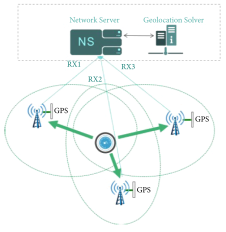
\includegraphics[width=0.5\linewidth]{Chapters/Figures/lorageo.JPG}}%
  \caption{Geolocation Architecture~\cite{Podevijn2018}}
  \label{fig:lora_Geo_Arch}
\end{figure}
\newpage
The LoRa Alliance claims that this feature achieves an estimation error of 20 to 200 m, as represented in figure~\ref{fig:lora_Geo_compare}. In~\cite{Fargas2017RL1} the~\gls{TDoA} method was evaluated, and the conclusion is  that is possible to get, a location accuracy of approximately 100 m for the stationary sender.\newline
\begin{figure}[htbp]
  \centering
    {\includegraphics[width=0.65\linewidth]{Chapters/Figures/lorageocopare.JPG}}%
  \caption{Geolocation Comparison~\cite{LoRa-Geo-White}}
  \label{fig:lora_Geo_compare}
\end{figure}
\newline In order to obtain a positioning for an NB-IoT device, one of the methods that could be used is  Observed Time Difference of Arrival (OTDoA) localization. For this method the base stations need to be synchronized and transmitting  a Positioning Reference Signal (PRS), which is then received by the device, in the event of PRS is unavailable, the cell-specific-reference-signal (CRS) can be used for the OTDoA. The  device needs to forwards the TOA of each  transmitting base station to a geolocation server, where the difference between these TOAs and the PRS, is used to perform the calculation of the estimated location~\cite{Hu2017}.\newline

\begin{figure}[htbp]
  \centering
    {\includegraphics[width=0.65\linewidth]{Chapters/Figures/NBOTDOA.JPG}}%
  \caption{NB-IoT OTDOA~\cite{Hu2017}}
  \label{fig:NBOTDOA}
\end{figure}


% subsection LPWAN Geolocation (end)
% section Geolocation (end)

%                               Section Related Work

\newpage
\section{Related Work} % (fold)
\label{sec:related_work}
%%%frase inicial


Most studies in the area of geolocation have focused on the use of a single technology, or technique. Then there are the ones that uses multiple technologies and techniques, but seems that do not explore so much the dynamic change of the working technology in functioning mode.
An analysis of related work shows in the first four examples, they focus only in different individual technologies and techniques. The last two focus either in multiple technologies, or multiple techniques, but as already emphasized, without taking into consideration the use of multiple techniques and technologies simultaneously.

In~\cite{Fargas2017RL1} an~\gls{IoT} tracking system is presented, using LoRA where the geolocation is calculated through a multilateration algorithm, on the gateways timestamp, with an accuracy of around 100m in statically test scenario.


In~\cite{RL3} the performance and accuracy of the Google API, for geolocation using WI-FI Aps is evaluated, the results in a urban environment, achieving a maximum accuracy of 20 meters, minimal 187 meters and median 39 meters.

In~\cite{DSouza2012RL4}, an  indoor localization monitoring system is presented and a wearable device was developed, using FleckTM-3 wireless sensor platform, with a position error of 1 to 3.5 meters. The main disadvantage of this work, is that only works indoors, and the technology is similar to ZigBee so only works for short range applications.

In~\cite{Tabbakha2018}, was developed an indoor position system based on Raspberry Pi and an MPU6050, used has BLE beacon, and with the use of Raspberry Pi as BLE scanner, measuring the RSSI, the results for indoor activity were 99\% of accuracy in knowing in which division the patience was.

In~\cite{Aernouts2018RL2} a dataset of messages was created from LoRa and Sigfox containing the~\gls{GPS} coordinates, and respective~\gls{RSSI}. The results of the median error in a urban scenario, were 514.83 meters for SigFox and 273.03 meters for LoRa.

In~\cite{Danebjer2018}, a Hybrid (Time of Flight and RSSI) approach for Geolocation system using LoRa,  and the results are similar to the work mentioned in~\cite{Aernouts2018RL2}, with a median error of 272 meters.

The work presented by the author improves the aforementioned solutions with an adaptive geolocation solution that combines the different methods, resulting in an overall location that provides the best results in terms of precision and performance wise, meeting the dynamic changes needed during the utilization scenarios.

% section related work (end)
